\section*{Лекція 10: Функції. Додаткові відомості}
 
 \subsection{Рекурсивні функції} 
\begin{frame}
\frametitle{Функція, що викликає саму себе}
Рекурсивна функція — функція, що викликає саму себе. При цьому функція розміщується в стек виклику функції. 
\begin{figure}
  \begin{center}
    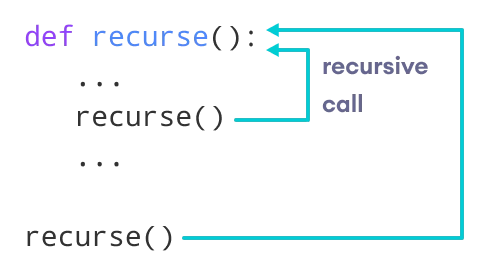
\includegraphics[width=0.5\textwidth,height=0.5\textheight]{pictures/recursion.png}
  \caption{Рекурсивна функція}
\label{function}
  \end{center}
\end{figure}
\end{frame}

\begin{frame}
\frametitle{Приклад рекурсивної функції}
\texttt{def recursive(value):}

\texttt{~~~~print(value)}

\texttt{~~~~if value < 4:}

\texttt{~~~~~~~~recursive(value)}

\texttt{~~~~print(value)}

\vspace{1cm}

Кількість внутрішніх викликів функції - глибина рекурсії.
\end{frame}

\subsection{Lambda-функції} 
\begin{frame}
\frametitle{Lambda-функція — анонімна функція}

\Large{\texttt{lambda param\_1, param\_2, ... : команда}}

\normalsize
\begin{itemize}
  \item lambda-функція автоматично повертає результат свого виконання (оператор return не потрібен);
  \item lambda-функція зазвичай присвоюється якійсь змінній; 
  \item lambda-функція може бути елементом будь-якої конструкції мови Python;
  \item всередині lambda-функції не можна виконувати присвоювання.
\end{itemize}

\end{frame}

\begin{frame}
\frametitle{Приклад використання lambda-функції}

\texttt{def get\_filter(a, filter=None):}

\texttt{~~~~ if filter is None:}

\texttt{~~~~~~~~return a}

\texttt{~~~~res = []}

\texttt{~~~~for x in a:}

\texttt{~~~~~~~~if filter(x):}

\texttt{~~~~~~~~~~~~res.append(x)}

\texttt{~~~~return res}

\texttt{print(get\_filter(a, filter=lambda x: x \% 2 == 0))}
\end{frame}

\subsection{Простір імен} 
\begin{frame}
\frametitle{Локальний та глобальний простір імен}
\underline{Локальний простір імен}: простір імен містить локальні імена всередині функції. Цей простір імен створюється під час виклику функції і продовжується, поки функція не повернеться.

\underline{Глобальний простір імен}: це простір імен, який включає імена різних імпортованих модулів, які ви використовуєте в проекті. Він створюється, коли модуль включений у проект, і існує до завершення виконання програми.

\end{frame}

\begin{frame}
\frametitle{Область видимості}
\underline{Локальна область видимості} є внутрішньою областю, яка містить список локальних імен, доступних у поточній функції.

\underline{Глобальна область  видимості} - область всіх функцій, що закривають. 

Пошук імені починається з найближчої області, що охоплює, і переміщається назовні.


\end{frame}

\begin{frame}
\frametitle{Команди global та nonlocal}

Щоб всередині функції змінити глобальну змінну \texttt{var} використовується команда \texttt{global var}.

Щоб всередині функції працювати зі змінною \texttt{var} із зовнішнього (локального) простору імен використовується команда \texttt{nonlocal var}.

\end{frame}

\subsection{Замикання} 
\begin{frame}
\frametitle{Визначення замикання}
Замикання (closure) - функція, яка знаходиться всередині іншої функції і посилається на змінні оголошені в тілі зовнішньої функції (вільні змінні).
\begin{figure}
  \begin{center}
    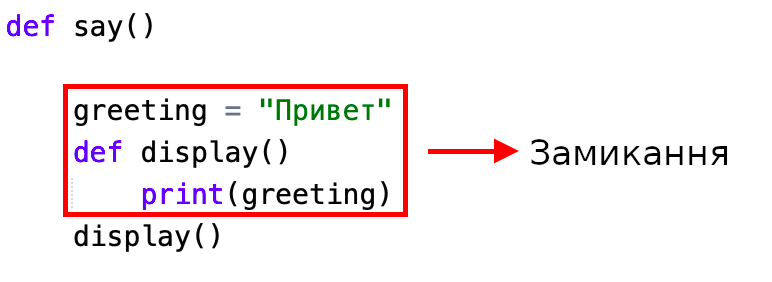
\includegraphics[width=0.5\textwidth,height=0.35\textheight]{pictures/closure.png}
  \caption{Замикання}
\label{function}
  \end{center}
\end{figure}

\end{frame}

\begin{frame}
\frametitle{Визначення замикання}


Внутрішня функція створюється щоразу під час виконання зовнішньої. Щоразу під час виклику зовнішньої функції відбувається створення нового екземпляра внутрішньої функції, з новими посиланнями на змінні зовнішньої функції.

Посилання на змінні зовнішньої функції дійсні всередині вкладеної функції до тих пір, поки працює вкладена функція, навіть якщо зовнішня функція закінчила роботу, і змінні вийшли з області видимості.
\end{frame}

\begin{frame}
\frametitle{Приклад замикання}
\large{
\texttt{def say\_name(name):}
 
\texttt{~~~~def say\_hello():}

\texttt{~~~~~~~~print("Hello, ", name)}

\texttt{~~~~return say\_hello}

\texttt{f = say\_name("Max")}
}
\normalsize
\end{frame}

\subsection{Декоратори} 
\begin{frame}
\frametitle{Що таке декоратор ?}
Декоратор - функція, яка використовується для зміни функції, використовується для додавання якогось функціоналу.

\begin{figure}
  \begin{center}
    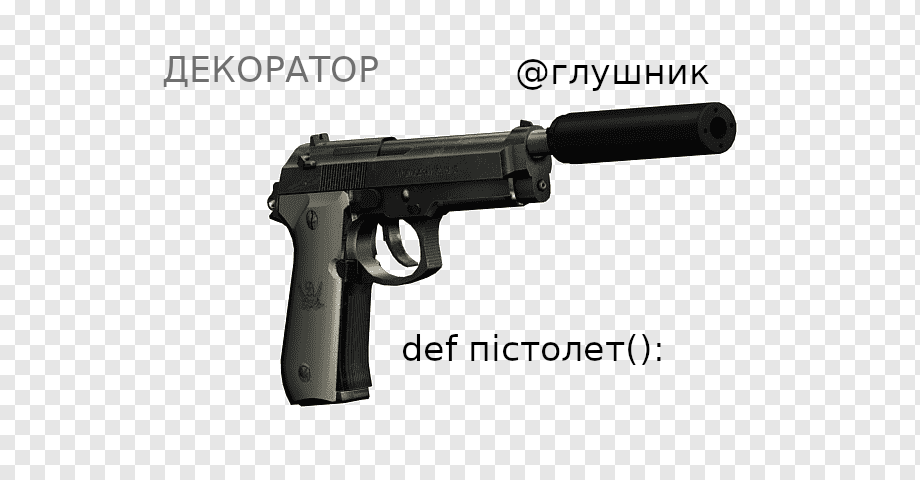
\includegraphics[width=0.5\textwidth,height=0.5\textheight]{pictures/decorator.png}
  \caption{Декоратор}
\label{function}
  \end{center}
\end{figure}


\end{frame}

\begin{frame}
\frametitle{Загальний вигляд декоратору}

\texttt{def func\_decorator(func):}

\texttt{~~~~def wrapper(*args, **kwargs):}

\texttt{~~~~~~~~operations before}

\texttt{~~~~~~~~func(*args, **kwargs)}

\texttt{~~~~~~~~operations after}

\texttt{~~~~return wrapper}

\texttt{some\_func = func\_decorator(some\_func)}

Для декорування можна перед визначенням функції написати \texttt{@func\_decorator}.
\end{frame}

\begin{frame}
\frametitle{Декоратор з параметром}

\texttt{def take\_parameter(p):}

\texttt{~~~~def func\_decorator(func):}

\texttt{~~~~~~~~def wrapper(*args, **kwargs):}

\texttt{~~~~~~~~~~~~operations before}

\texttt{~~~~~~~~~~~~func(p, *args, **kwargs)}

\texttt{~~~~~~~~~~~~operations after}

\texttt{~~~~~~~~return wrapper}

\texttt{~~~~return func\_decorator}

Для декорування можна перед визначенням функції написати \texttt{@take\_parameter(p)}.
\end{frame}
